\documentclass[12pt, a4paper]{article}

\usepackage[utf8]{inputenc}
\usepackage[pdftex]{graphicx}
\usepackage{booktabs}
\usepackage{amsmath}
\usepackage{amssymb}
\usepackage[left=2.5cm,right=2.5cm,top=3cm,bottom=3.5cm]{geometry}
\usepackage{indentfirst}
\usepackage[activate={true,nocompatibility},final,tracking=true,kerning=true,spacing=true,factor=1100,stretch=10,shrink=10]{microtype}
\usepackage{float}

\renewcommand{\figurename}{Slika}

\microtypecontext{spacing=nonfrench}

\allowdisplaybreaks

\title{Neizrazito, evolucijsko i neuroračunarstvo:\\
  izvješće uz 6. laboratorijsku vježbu - sustav ANFIS}

\author{Lovre Mrčela}

\date{7. siječnja 2017.}

\begin{document}

\maketitle

\section*{Derivacije pogreške s obzirom na parametre mreže}

Ukupna pogreška $E$ je:

$$ E = \dfrac{1}{2} \sum_{n=1}^{N} \left( o^{(n)} - t^{(n)} \right)^2, $$
gdje je $N$ broj pravila, $o^{(n)}$ dobiveni izlaz iz sustava, a $t^{(n)}$ očekivani izlaz iz sustava, za $n$-ti primjer.

$n$-ti izlaz $o^{(n)}$ je:

$$ o^{(n)} = \sum_{m=1}^{M} \widetilde{w}_m f_m \left( x^{(n)}, y^{(n)}; p_m, q_m, r_m \right), $$
gdje je $\widetilde{w}_m$ pripadna normirana težina, a $f_m$ prijenosna funkcija s parametrima $p_m$, $q_m$, i $r_m$, $m$-tog pravila; $x^{(n)}$ i $y^{(n)}$ su vrijednosti $n$-tog primjera u ovom zadatku.

Prijenosna funkcija $m$-tog pravila $f_m$ je, u ovom zadatku, linearna kombinacija vrijednosti $x^{(n)}$ i $y^{(n)}$ $n$-tog ulaza:

$$ f_m \left( x^{(n)}, y^{(n)}; p_m, q_m, r_m \right) = p_m x^{(n)} + q_m y^{(n)} + r_m. $$


Normirana težina $m$-tog pravila $\widetilde{w}_m$ je:

$$ \widetilde{w}_m = \dfrac{w_m}{\sum_{k=1}^{M} w_k}. $$

Nenormirana težina $m$-tog pravila $w_m$ jednaka je $t$-normi mjera pripadnosti $n$-tog ulaznog primjera paru neizrazitih skupova $(A_m, B_m)$. U ovom zadatku zadana $t$-norma je algebarski produkt $\left( \cdot \right)$, pa je nenormirana težina $w_m$:

$$ w_m = \mu_{A_m} \left( x^{(n)} \right) \cdot \mu_{B_m} \left( y^{(n)} \right), $$
gdje je $\mu_{X_m} \left( z \right)$ mjera pripadnosti elementa $z$ neizrazitom skupu $X_m$ $m$-tog pravila.

Mjere pripadnosti $\mu_{X_m} \left( z \right)$ u ovom zadatku modelirane su parametriziranim sigmoidalnim funkcijama s parametrima $a_{X_m}$ i $b_{X_m}$:

$$ \mu_{X_m} \left( z; a_{X_m}, b_{X_m} \right) = \dfrac{1}{1 + e^{-b_{X_m} \left( z - a_{X_m} \right)}}. $$

Za $m$-to pravilo postoji 7 parametara koje je potrebno trenirati na zadanom skupu podataka: $p_m$, $q_m$, $r_m$, $a_{A_m}$, $a_{B_m}$, $b_{A_m}$, i $b_{B_m}$. Ukupno je $7 M$ parametara, gdje je M broj pravila.

Derivacija ukupne pogreške s obzirom na izlaz iz sustava $o^{(n)}$ za $n$-ti primjer je:

$$ \dfrac{\partial E}{\partial o^{(n)}} = o^{(n)} - t^{(n)}. $$

Derivacija izlaza $o^{(n)}$ za $n$-ti primjer po prijenosnoj funkciji $f_m$ $m$-tog pravila je:

$$ \dfrac{\partial o^{(n)}}{\partial f_m} = \widetilde{w}_m. $$

Derivacije prijenosne funkcije $f_m$ $m$-tog pravila po parametrima $p_m$, $q_m$, i $r_m$, za $n$-ti primjer, su:

$$
  \dfrac{\partial f_m}{\partial p_m} = x^{(n)}, \qquad
  \dfrac{\partial f_m}{\partial q_m} = y^{(n)}, \qquad
  \dfrac{\partial f_m}{\partial r_m} = 1.
$$

Derivacije nenormirane težine $w_m$ $m$-tog pravila po mjerama pripadnosti neizrazitim skupovima $\mu_{A_m}$ i $\mu_{B_m}$, za $n$-ti primjer su:

$$
  \dfrac{\partial w_m}{\partial \mu_{A_m}}
  = \mu_{B_m} \left( y^{(n)}; a_{B_m}, b_{B_m} \right), \qquad
  \dfrac{\partial w_m}{\partial \mu_{B_m}}
  = \mu_{A_m} \left( x^{(n)}; a_{A_m}, b_{A_m} \right),
$$

Budući da je normirana težina $\widetilde{w}_j$ funkcija svih težina $\left\{ w_m \right\}_{m=1}^{M}$, derivacije normiranih težina $w_j$ $j$-tog pravila po nenormiranoj težini $w_m$ $m$-tog pravila nisu 0 te ih je potrebno izračunati:

\begin{align*}
  \dfrac{\partial \widetilde{w}_j}{\partial w_{m}} &= \begin{cases}
    \dfrac{\left(\sum_{k=1}^{M} w_k \right) - w_m}{\left( \sum_{k=1}^{M} w_k \right)^2}, & m = j, \\
    \dfrac{-w_j}{\left( \sum_{k=1}^{M} w_k \right)^2}, & m \ne j,
  \end{cases} \\
  &= \dfrac{\delta_{m, j} \left(\sum_{k=1}^{M} w_k \right) - w_j}{\left( \sum_{k=1}^{M} w_k \right)^2},
\end{align*}
uz Kroneckerov delta $\delta_{i, j}$:

\begin{align*}
  \delta_{i, j} &= \begin{cases}
    1, & i = j, \\
    0, & i \ne j,
\end{cases}
\end{align*}
a ukupna derivacija izlaza iz sustava $o^{(n)}$ za $n$-ti primjer po težini $w_m$ $m$-tog pravila je:

\begin{align*}
  \dfrac{\partial o^{(n)}}{\partial w_m} &=
  \sum_{j=1}^{M} \dfrac{\partial o^{(n)}}{\partial \widetilde{w}_j}
    \dfrac{\partial\widetilde{w}_j}{\partial w_m} =
  \sum_{j=1}^{M} f_j  \left( x^{(n)}, y^{(n)}; p_j, q_j, r_j \right)
  \dfrac{ \delta_{m, j} \left(\sum_{k=1}^{M} w_k \right) - w_j}{\left( \sum_{k=1}^{M} w_k \right)^2} \\
  &= \dfrac{
     \sum_{j=1}^{M} \delta_{m, j} \left( \left(\sum_{k=1}^{M} w_k \right) - w_j \right)
     f_j  \left( x^{(n)}, y^{(n)}; p_j, q_j, r_j \right)}
     {\left( \sum_{k=1}^{M} w_k \right)^2} \\
  &= \dfrac{
    \sum_{j=1}^{M} \delta_{m, j} \left(\sum_{k=1}^{M} w_k \right)
    f_j \left( x^{(n)}, y^{(n)}; p_j, q_j, r_j \right)
    - \sum_{j=1}^{M} w_j f_j \left( x^{(n)}, y^{(n)}; p_j, q_j, r_j \right)}
  {\left( \sum_{k=1}^{M} w_k \right)^2} \\
  &= \dfrac{
    \left(\sum_{k=1}^{M} w_k \right)
    f_m \left( x^{(n)}, y^{(n)}; p_m, q_m, r_m \right)
    - \sum_{j=1}^{M} w_j f_j \left( x^{(n)}, y^{(n)}; p_j, q_j, r_j \right)}
  {\left( \sum_{k=1}^{M} w_k \right)^2} \\
  &= \dfrac{
    \sum_{k=1}^{M} w_k
    \left( f_m \left( x^{(n)}, y^{(n)}; p_m, q_m, r_m \right)
    - f_k \left( x^{(n)}, y^{(n)}; p_k, q_k, r_k \right)\right)}
  {\left( \sum_{k=1}^{M} w_k \right)^2} \\
\end{align*}

Derivacije mjere pripadnosti $\mu_{X_m}$ elementa $z^{(n)}$ neizrazitom skupu $X_m$ $m$-tog pravila po parametrima $a_{X_m}$ i $b_{X_m}$ su:

\begin{align*}
  \dfrac{\partial \mu_{X_m}}{\partial a_{X_m}}
  &= \dfrac{-1}{\left( 1 + e^{-b_{X_m}\left( z^{(n)} - a_{X_m} \right)} \right)^2} \cdot
    e^{-b_{X_m}\left( z^{(n)} - a_{X_m} \right)} \cdot (-b) \\
  &= -b \cdot \mu_{X_m} \left( z^{(n)}; a_{X_m}, b_{X_m} \right) \cdot \left( 1 - \mu_{X_m} \left( z^{(n)}; a_{X_m}, b_{X_m} \right) \right) \\ \\
  \dfrac{\partial \mu_{X_m}}{\partial b_{X_m}}
  &= \dfrac{-1}{\left( 1 + e^{-b_{X_m}\left( z^{(n)} - a_{X_m} \right)} \right)^2} \cdot
  e^{-b_{X_m}\left( z^{(n)} - a_{X_m} \right)} \cdot (-(x - a)) \\
  &= (x - a) \cdot \mu_{X_m} \left( z^{(n)}; a_{X_m}, b_{X_m} \right) \cdot \left( 1 - \mu_{X_m} \left( z^{(n)}; a_{X_m}, b_{X_m} \right) \right)
\end{align*}

Konačno, tražene derivacije ukupne pogreške s obzirom na sve parametre sustava za $m$-to pravilo i $n$-ti ulazni primjer su:

\begin{align*}
  \dfrac{\partial E}{\partial p_m} &= 
    \dfrac{\partial E}{\partial o^{(n)}} 
    \dfrac{\partial o^{(n)}}{\partial f_m}
    \dfrac{\partial f_m}{\partial p_m} =
    \left( o^{(n)} - t^{(n)} \right) \cdot
    \widetilde{w}_m \cdot x^{(n)}, \\ \\
  \dfrac{\partial E}{\partial q_m} &= 
    \dfrac{\partial E}{\partial o^{(n)}} 
    \dfrac{\partial o^{(n)}}{\partial f_m}
    \dfrac{\partial f_m}{\partial q_m} =
    \left( o^{(n)} - t^{(n)} \right) \cdot
    \widetilde{w}_m \cdot y^{(n)}, \\ \\
  \dfrac{\partial E}{\partial r_m} &= 
    \dfrac{\partial E}{\partial o^{(n)}} 
    \dfrac{\partial o^{(n)}}{\partial f_m}
    \dfrac{\partial f_m}{\partial r_m} =
    \left( o^{(n)} - t^{(n)} \right) \cdot
    \widetilde{w}_m, \\ \\
  \dfrac{\partial E}{\partial a_{A_m}} &=
    \dfrac{\partial E}{\partial o^{(n)}} 
    \dfrac{\partial o^{(n)}}{\partial w_m}
    \dfrac{\partial w_m}{\mu_{A_m}}
    \dfrac{\partial \mu_{A_m}}{\partial a_{A_m}}, \\ &=
    \left( o^{(n)} - t^{(n)} \right) \cdot
    \dfrac{
      \sum_{k=1}^{M} w_k
      \left( f_m \left( x^{(n)}, y^{(n)}; p_m, q_m, r_m \right)
      - f_k \left( x^{(n)}, y^{(n)}; p_k, q_k, r_k \right)\right)}
    {\left( \sum_{k=1}^{M} w_k \right)^2} \cdot \\ &
    \mu_{B_m} \left( y^{(n)}; a_{B_m}, b_{B_m} \right) \cdot
    (-b) \cdot \mu_{A_m} \left( x^{(n)}; a_{A_m}, b_{A_m} \right) \cdot \left( 1 - \mu_{A_m} \left( x^{(n)}; a_{A_m}, b_{A_m} \right) \right), \\ \\
  \dfrac{\partial E}{\partial b_{A_m}} &= 
    \dfrac{\partial E}{\partial o^{(n)}} 
    \dfrac{\partial o^{(n)}}{\partial w_m}
    \dfrac{\partial w_m}{\mu_{A_m}}
    \dfrac{\partial \mu_{A_m}}{\partial b_{A_m}}, \\ &= 
    \left( o^{(n)} - t^{(n)} \right) \cdot
    \dfrac{
      \sum_{k=1}^{M} w_k
      \left( f_m \left( x^{(n)}, y^{(n)}; p_m, q_m, r_m \right)
      - f_k \left( x^{(n)}, y^{(n)}; p_k, q_k, r_k \right)\right)}
    {\left( \sum_{k=1}^{M} w_k \right)^2} \cdot \\ &
    \mu_{B_m} \left( y^{(n)}; a_{B_m}, b_{B_m} \right) \cdot 
    (x - a) \cdot \mu_{A_m} \left( x^{(n)}; a_{A_m}, b_{A_m} \right) \cdot \left( 1 - \mu_{A_m} \left( x^{(n)}; a_{A_m}, b_{A_m} \right) \right), \\ \\
  \dfrac{\partial E}{\partial a_{B_m}} &= 
    \dfrac{\partial E}{\partial o^{(n)}} 
    \dfrac{\partial o^{(n)}}{\partial w_m}
    \dfrac{\partial w_m}{\mu_{B_m}}
    \dfrac{\partial \mu_{B_m}}{\partial a_{B_m}}, \\ &= 
    \left( o^{(n)} - t^{(n)} \right) \cdot
    \dfrac{
      \sum_{k=1}^{M} w_k
      \left( f_m \left( x^{(n)}, y^{(n)}; p_m, q_m, r_m \right)
      - f_k \left( x^{(n)}, y^{(n)}; p_k, q_k, r_k \right)\right)}
    {\left( \sum_{k=1}^{M} w_k \right)^2} \cdot \\ &
    \mu_{A_m} \left( x^{(n)}; a_{A_m}, b_{A_m} \right) \cdot
    (-b) \cdot \mu_{B_m} \left( y^{(n)}; a_{B_m}, b_{B_m} \right) \cdot \left( 1 - \mu_{B_m} \left( y^{(n)}; a_{B_m}, b_{B_m} \right) \right), \\ \\
  \dfrac{\partial E}{\partial b_{B_m}} &=
    \dfrac{\partial E}{\partial o^{(n)}} 
    \dfrac{\partial o^{(n)}}{\partial w_m}
    \dfrac{\partial w_m}{\mu_{B_m}}
    \dfrac{\partial \mu_{B_m}}{\partial b_{B_m}}, \\ &=
    \left( o^{(n)} - t^{(n)} \right) \cdot
    \dfrac{
      \sum_{k=1}^{M} w_k
      \left( f_m \left( x^{(n)}, y^{(n)}; p_m, q_m, r_m \right)
      - f_k \left( x^{(n)}, y^{(n)}; p_k, q_k, r_k \right)\right)}
    {\left( \sum_{k=1}^{M} w_k \right)^2} \cdot \\ &
    \mu_{A_m} \left( x^{(n)}; a_{A_m}, b_{A_m} \right) \cdot
    (x - a) \cdot \mu_{B_m} \left( y^{(n)}; a_{B_m}, b_{B_m} \right) \cdot \left( 1 - \mu_{B_m} \left( y^{(n)}; a_{B_m}, b_{B_m} \right) \right).
\end{align*}

\section*{Pogreška tijekom treniranja}

\begin{figure}[H]
  \centering
  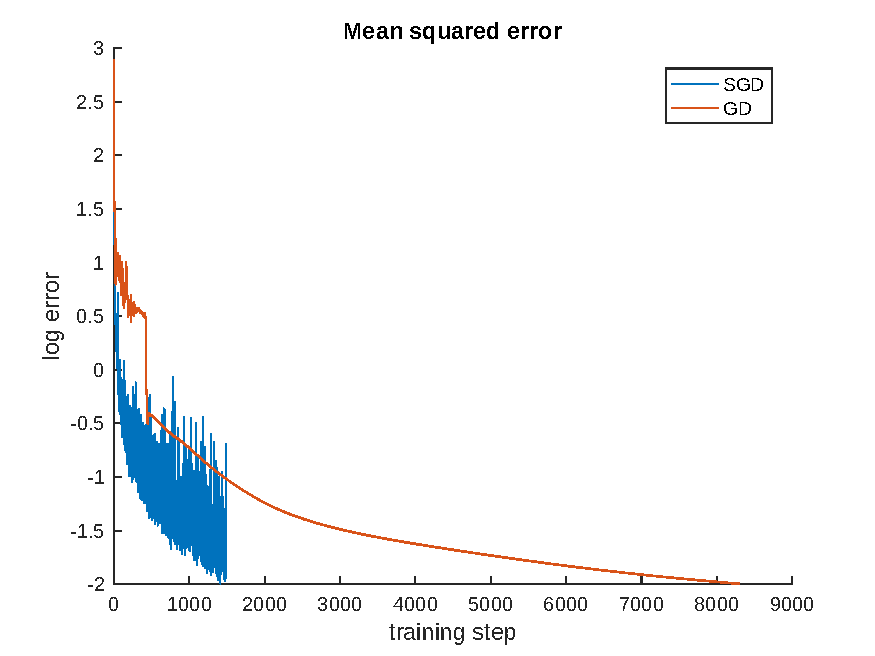
\includegraphics[width=\linewidth]{graf_normalna.pdf}
  \caption{Pogreška za vrijeme treniranja uz umjerenu stopu učenja $\eta=0.01$.}
\end{figure}

\begin{figure}[H]
  \centering
  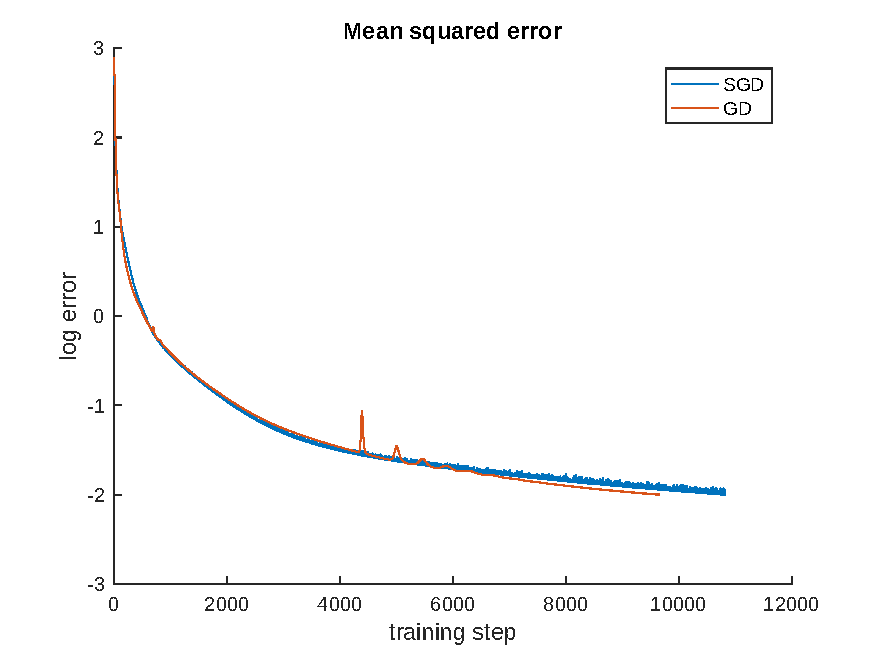
\includegraphics[width=\linewidth]{graf_niska.pdf}
  \caption{Pogreška za vrijeme treniranja uz nisku stopu učenja $\eta=0.001$.}
\end{figure}

\begin{figure}[H]
  \centering
  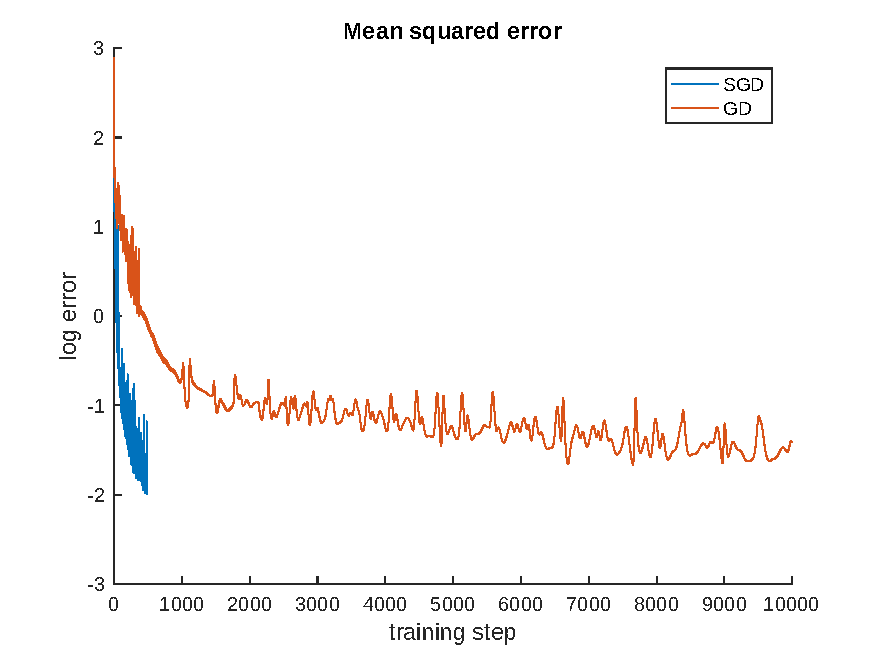
\includegraphics[width=\linewidth]{graf_visoka.pdf}
  \caption{Pogreška za vrijeme treniranja uz visoku stopu učenja $\eta=0.05$.}
\end{figure}

\section*{Pogreške na primjerima}

\begin{figure}[H]
  \centering
  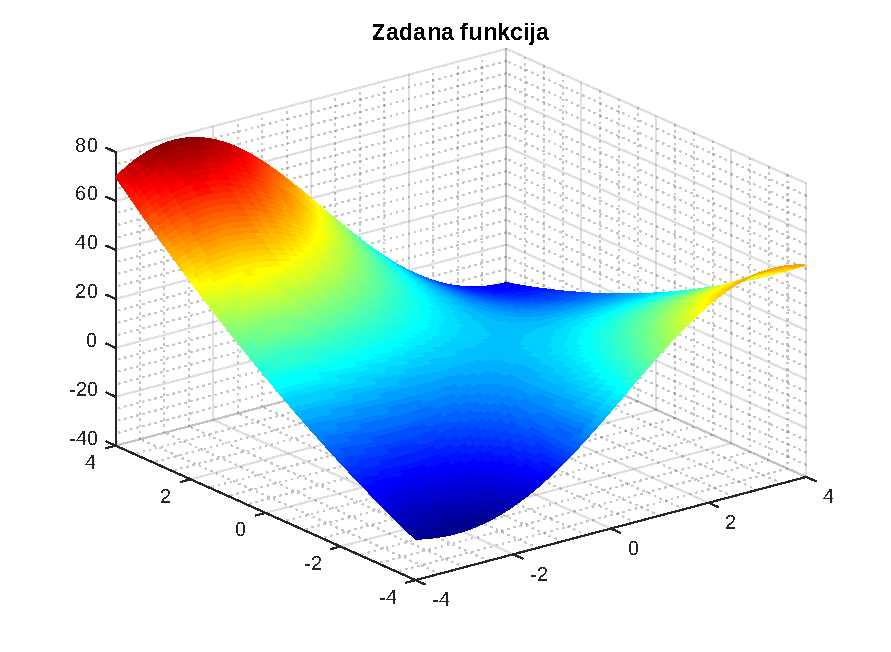
\includegraphics[width=\linewidth]{zadana.pdf}
  \caption{Zadana funkcija $\left( \left( x - 1 \right)^2 - \left(y + 2\right)^2 - 5 x y + 3 \right) \cdot \cos^2\left( \frac{x}{5} \right)$.}
\end{figure}

\begin{figure}[H]
  \centering
  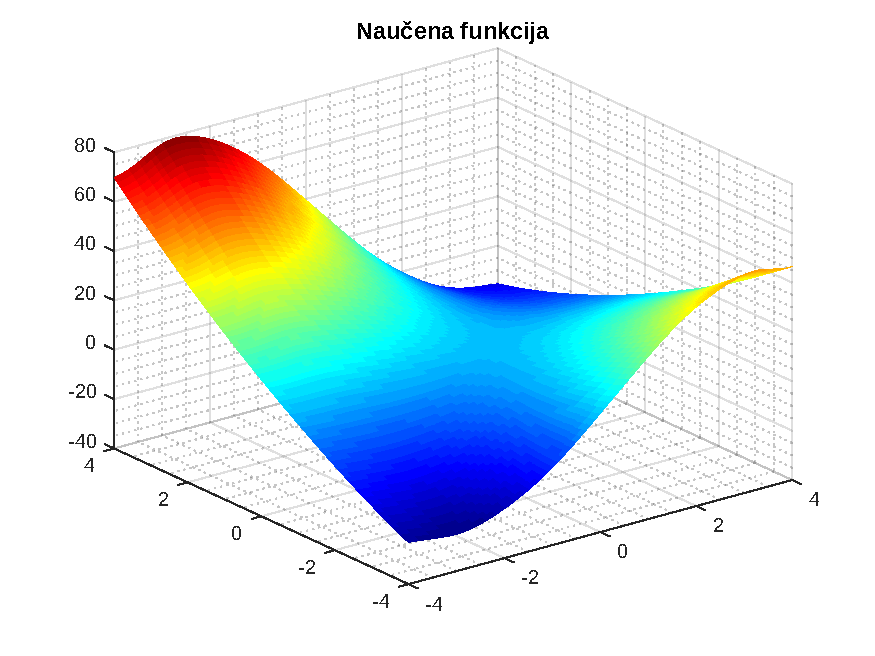
\includegraphics[width=\linewidth]{naucena.pdf}
  \caption{Naučena funkcija.}
\end{figure}

\begin{figure}[H]
  \centering
  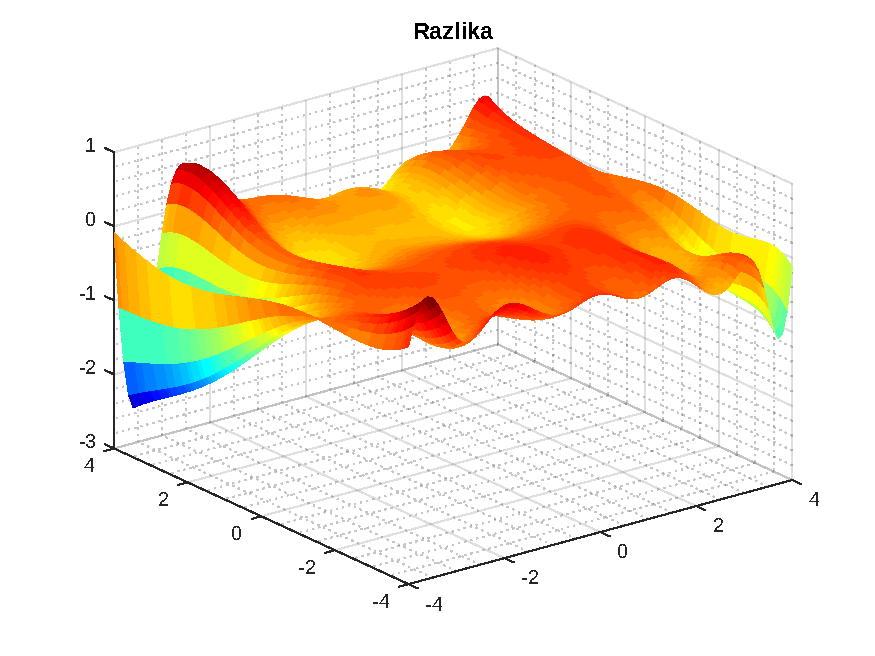
\includegraphics[width=\linewidth]{razlika.pdf}
  \caption{Razlika zadane i naučene funkcije.}
\end{figure}

\section*{Mjere pripadnosti u naučenom sustavu}

\begin{figure}[H]
  \centering
  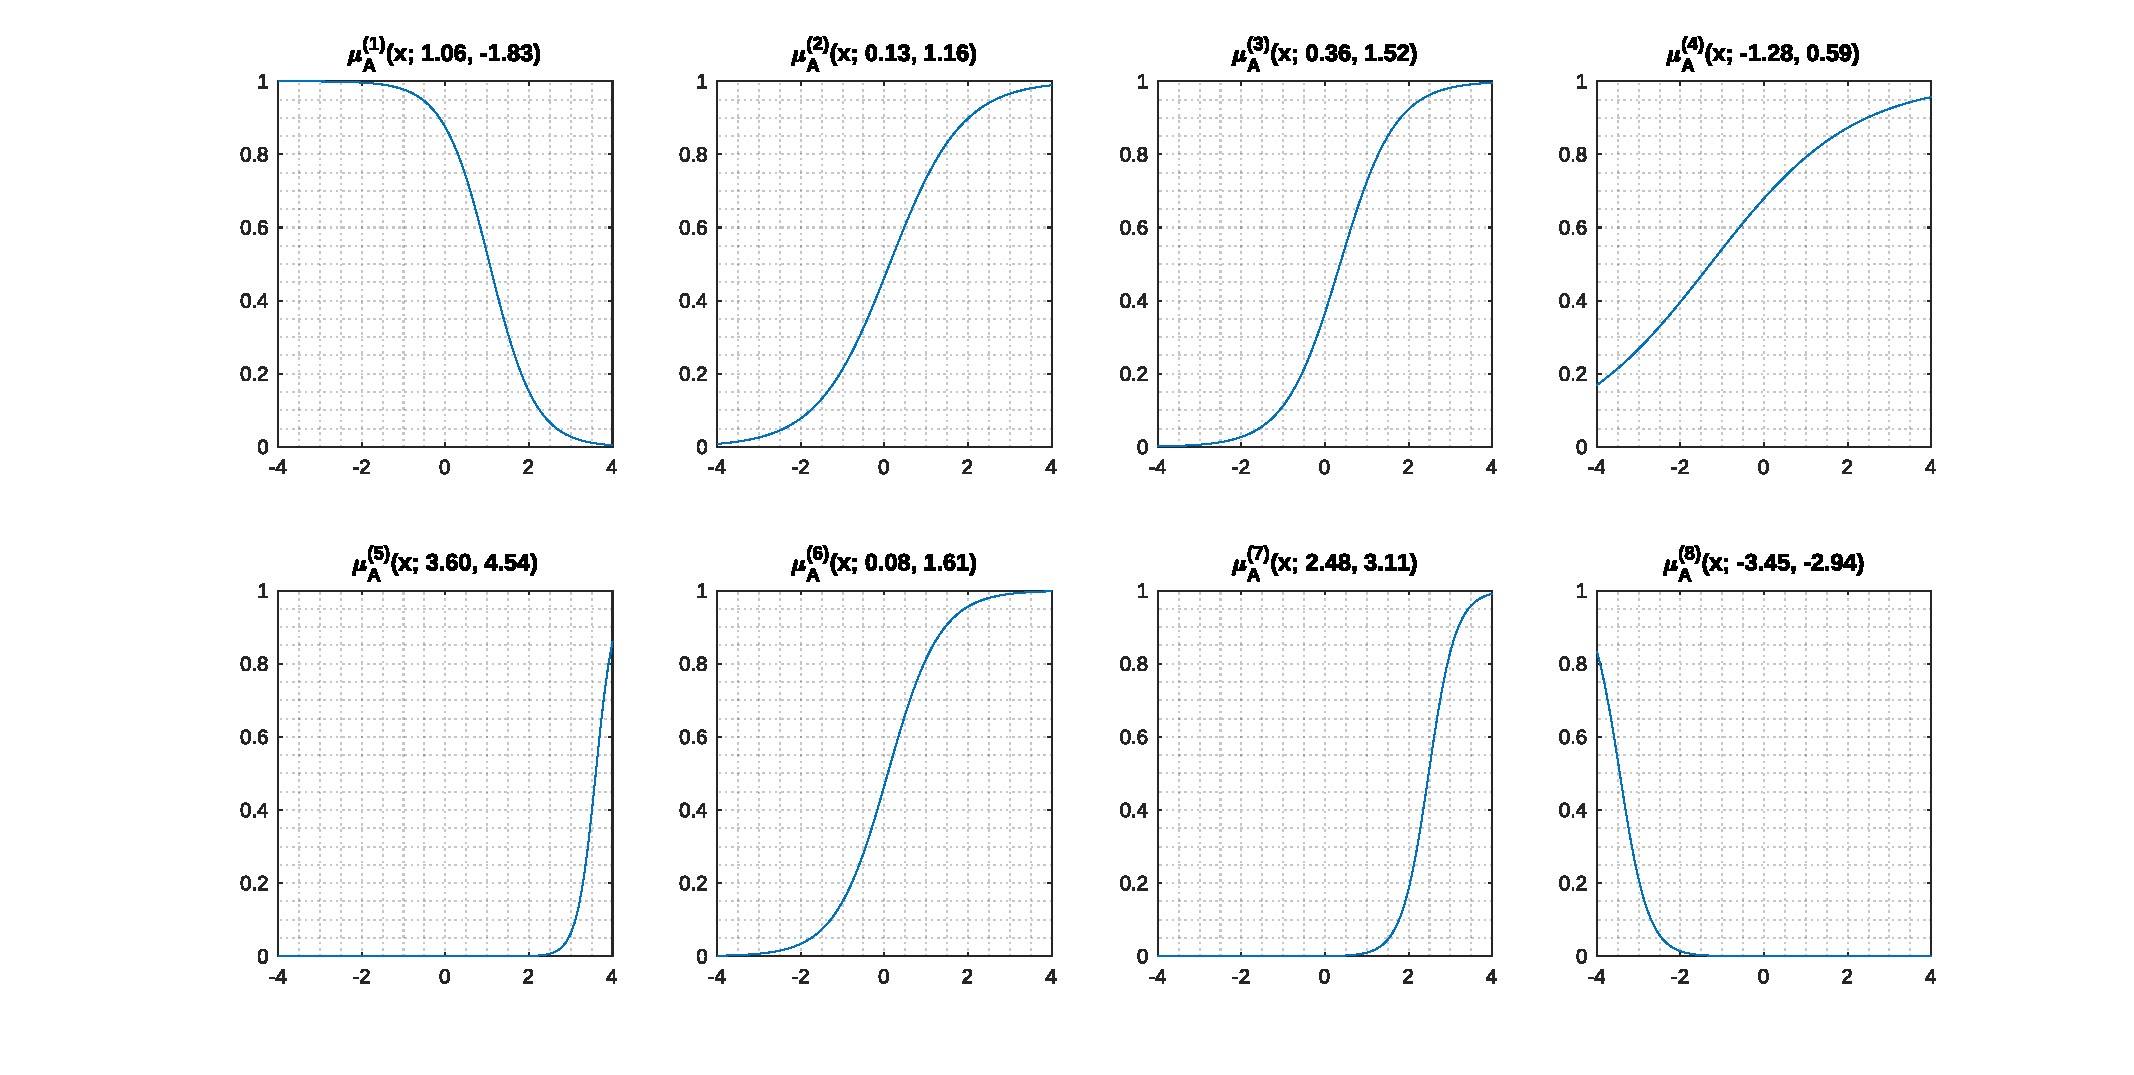
\includegraphics[width=\linewidth]{mem_A.pdf}
  \caption{Mjere pripadnosti neizrazitom skupu $A$.}
\end{figure}

\begin{figure}[H]
  \centering
  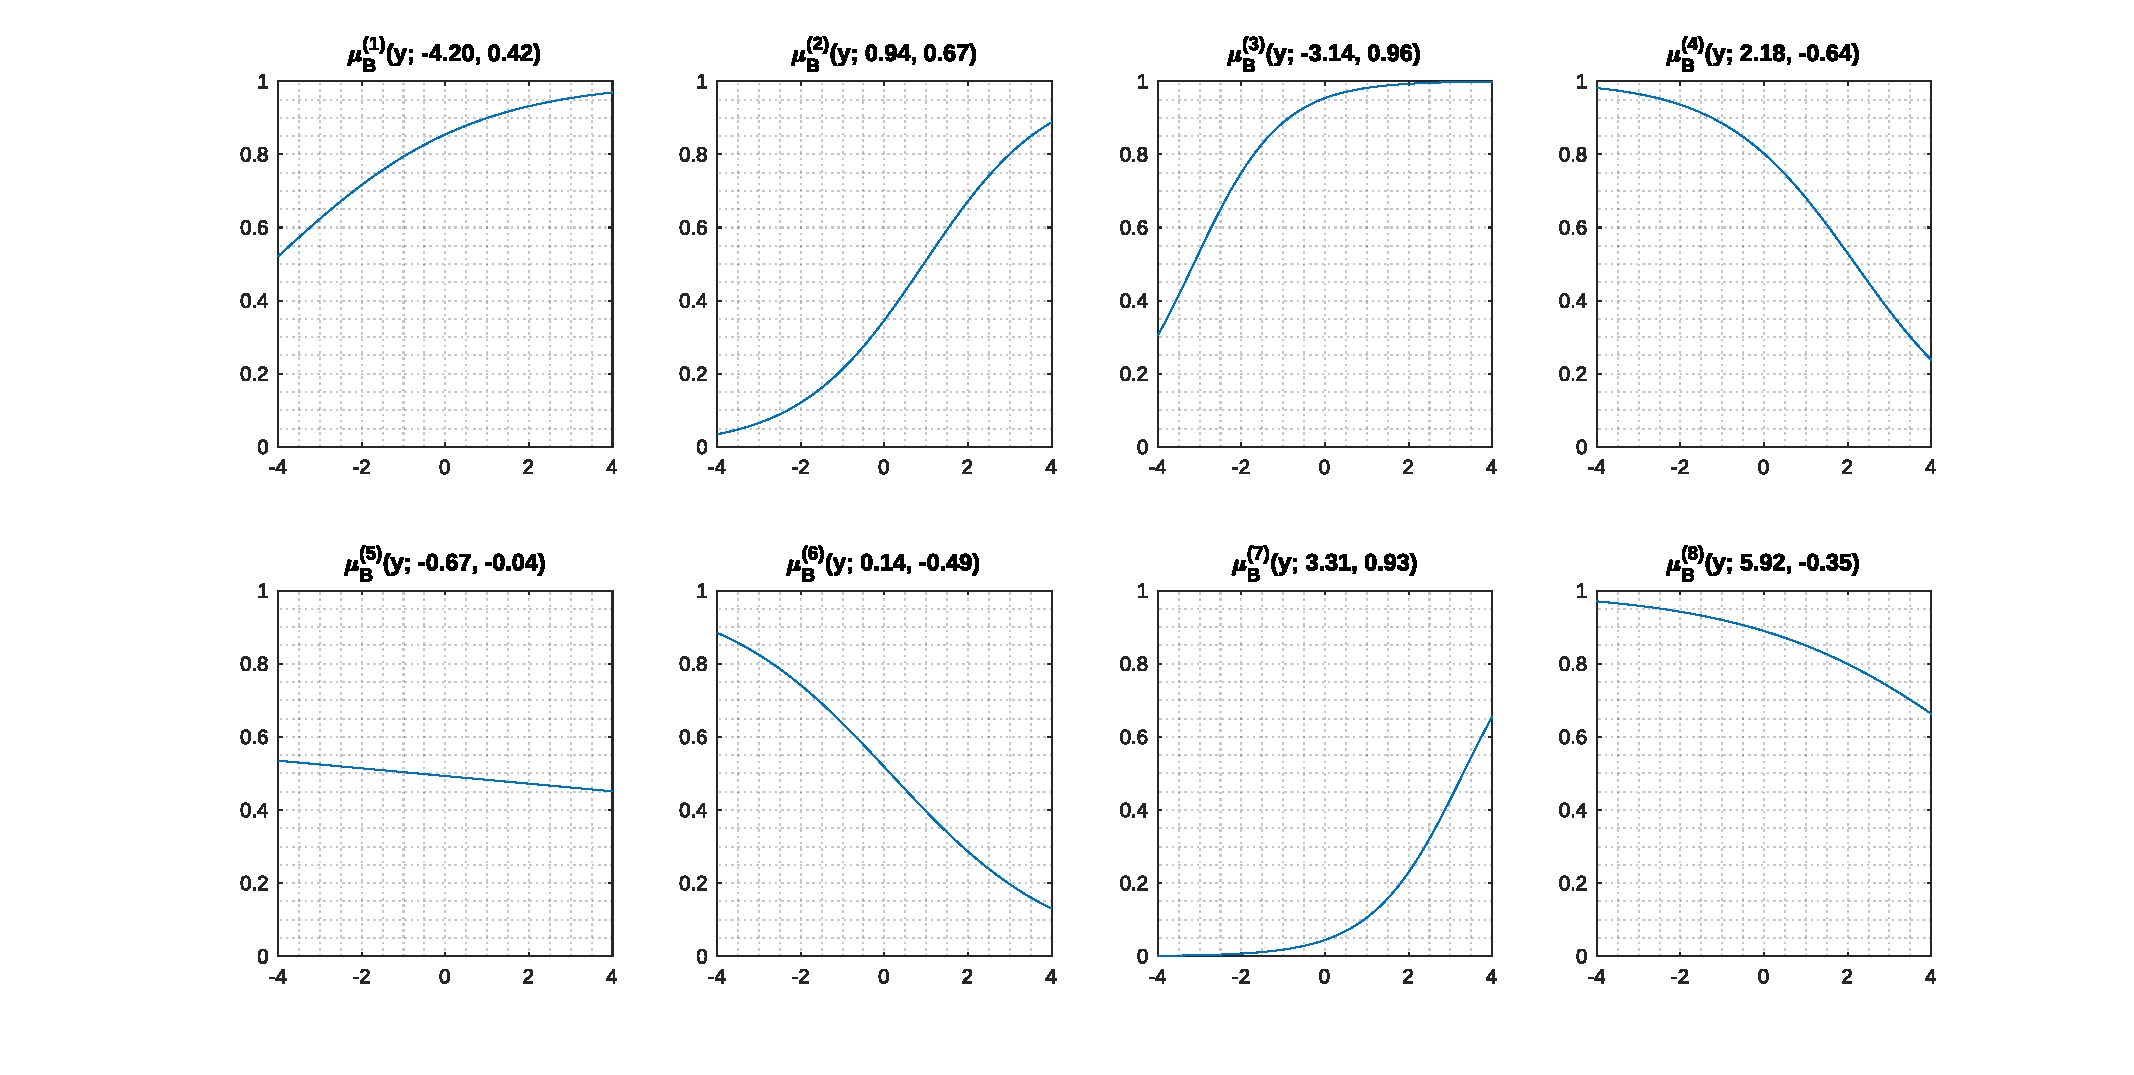
\includegraphics[width=\linewidth]{mem_B.pdf}
  \caption{Mjere pripadnosti neizrazitom skupu $B$.}
\end{figure}

\begin{figure}[H]
  \centering
  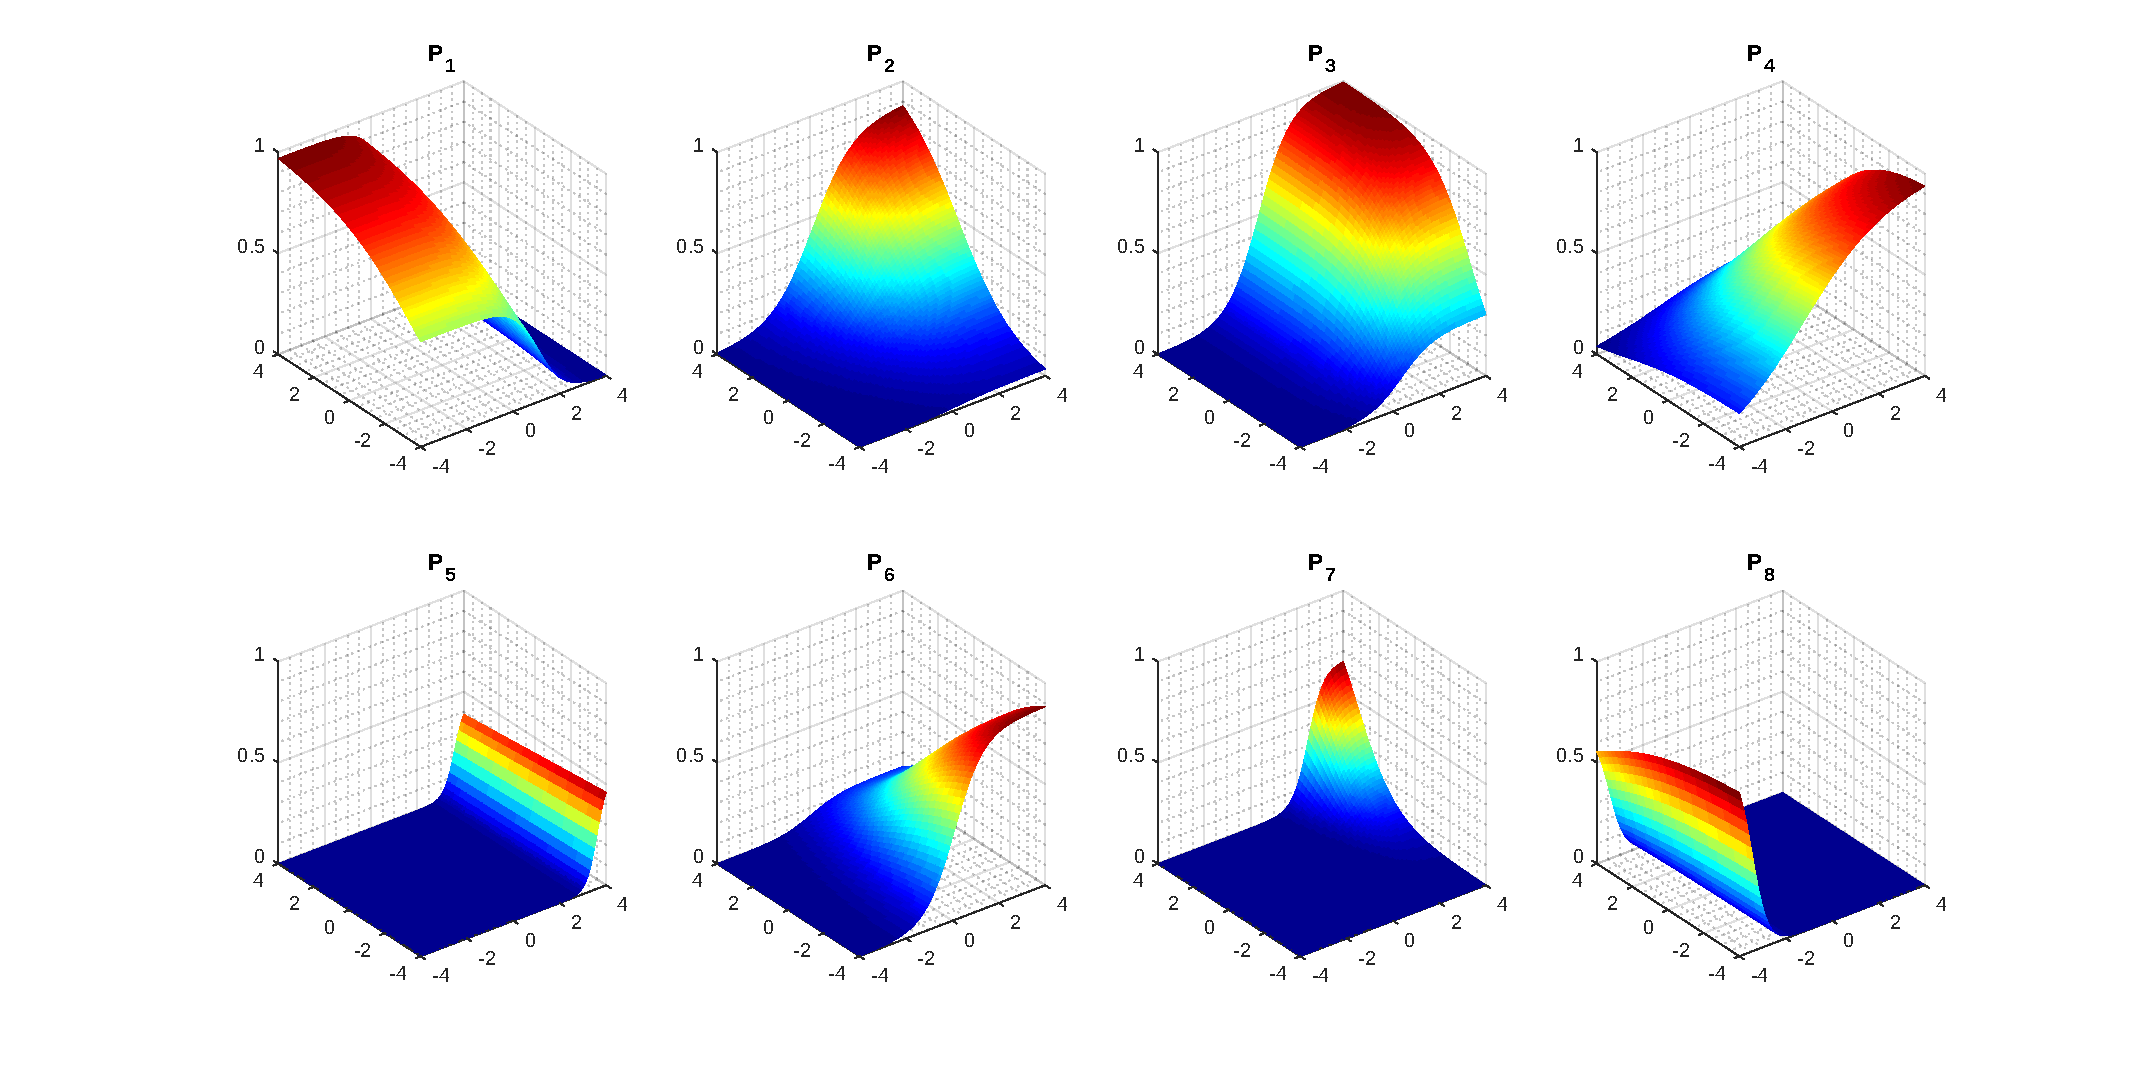
\includegraphics[width=\linewidth]{P.pdf}
  \caption{$t$-norma (algebarski produkt) mjera pripadnosti neizrazitim skupovima $A$ i $B$.}
\end{figure}

\section*{Prijenosne funkcije u naučenom sustavu}

\begin{figure}[H]
  \centering
  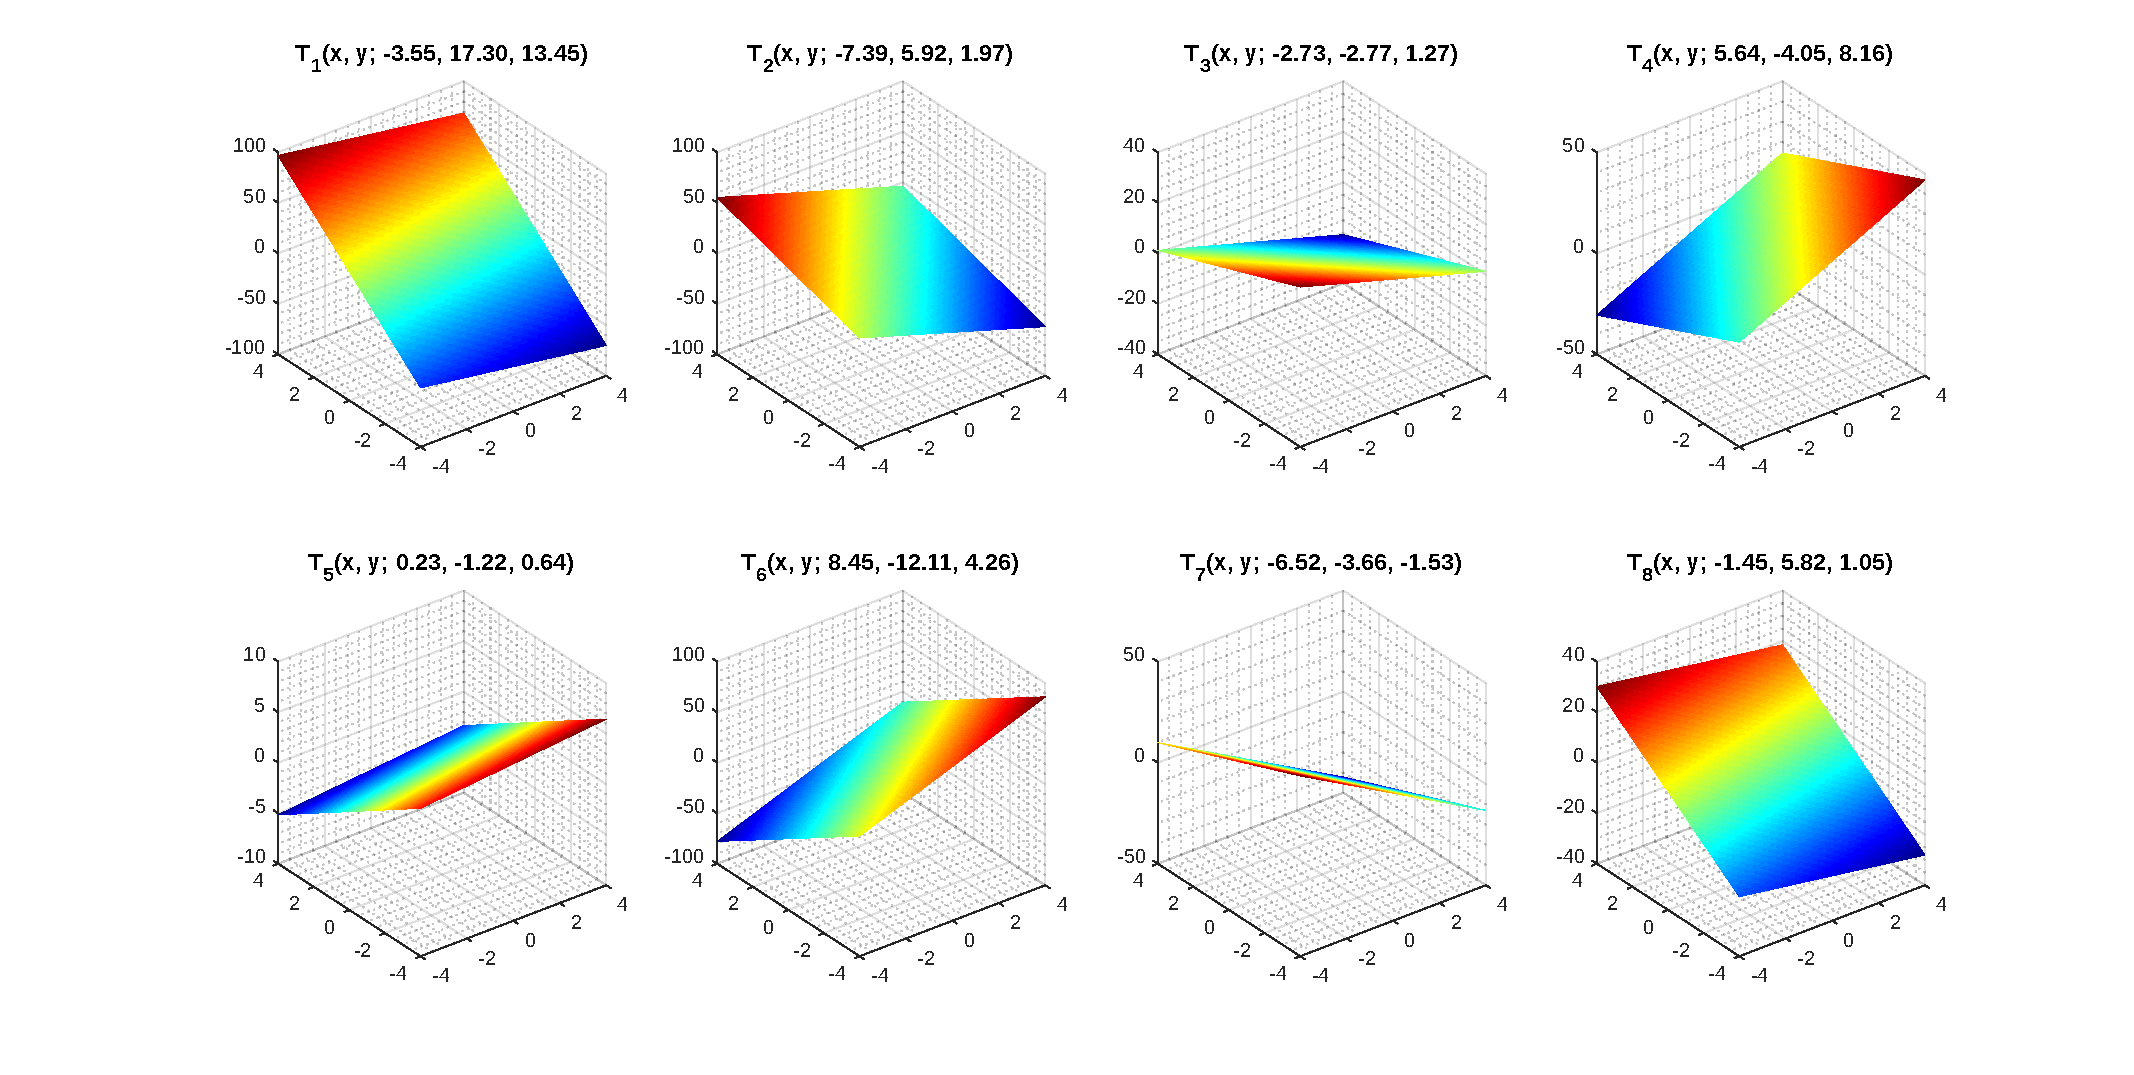
\includegraphics[width=\linewidth]{T.pdf}
  \caption{Prijenosne funkcije.}
\end{figure}

\begin{figure}[H]
  \centering
  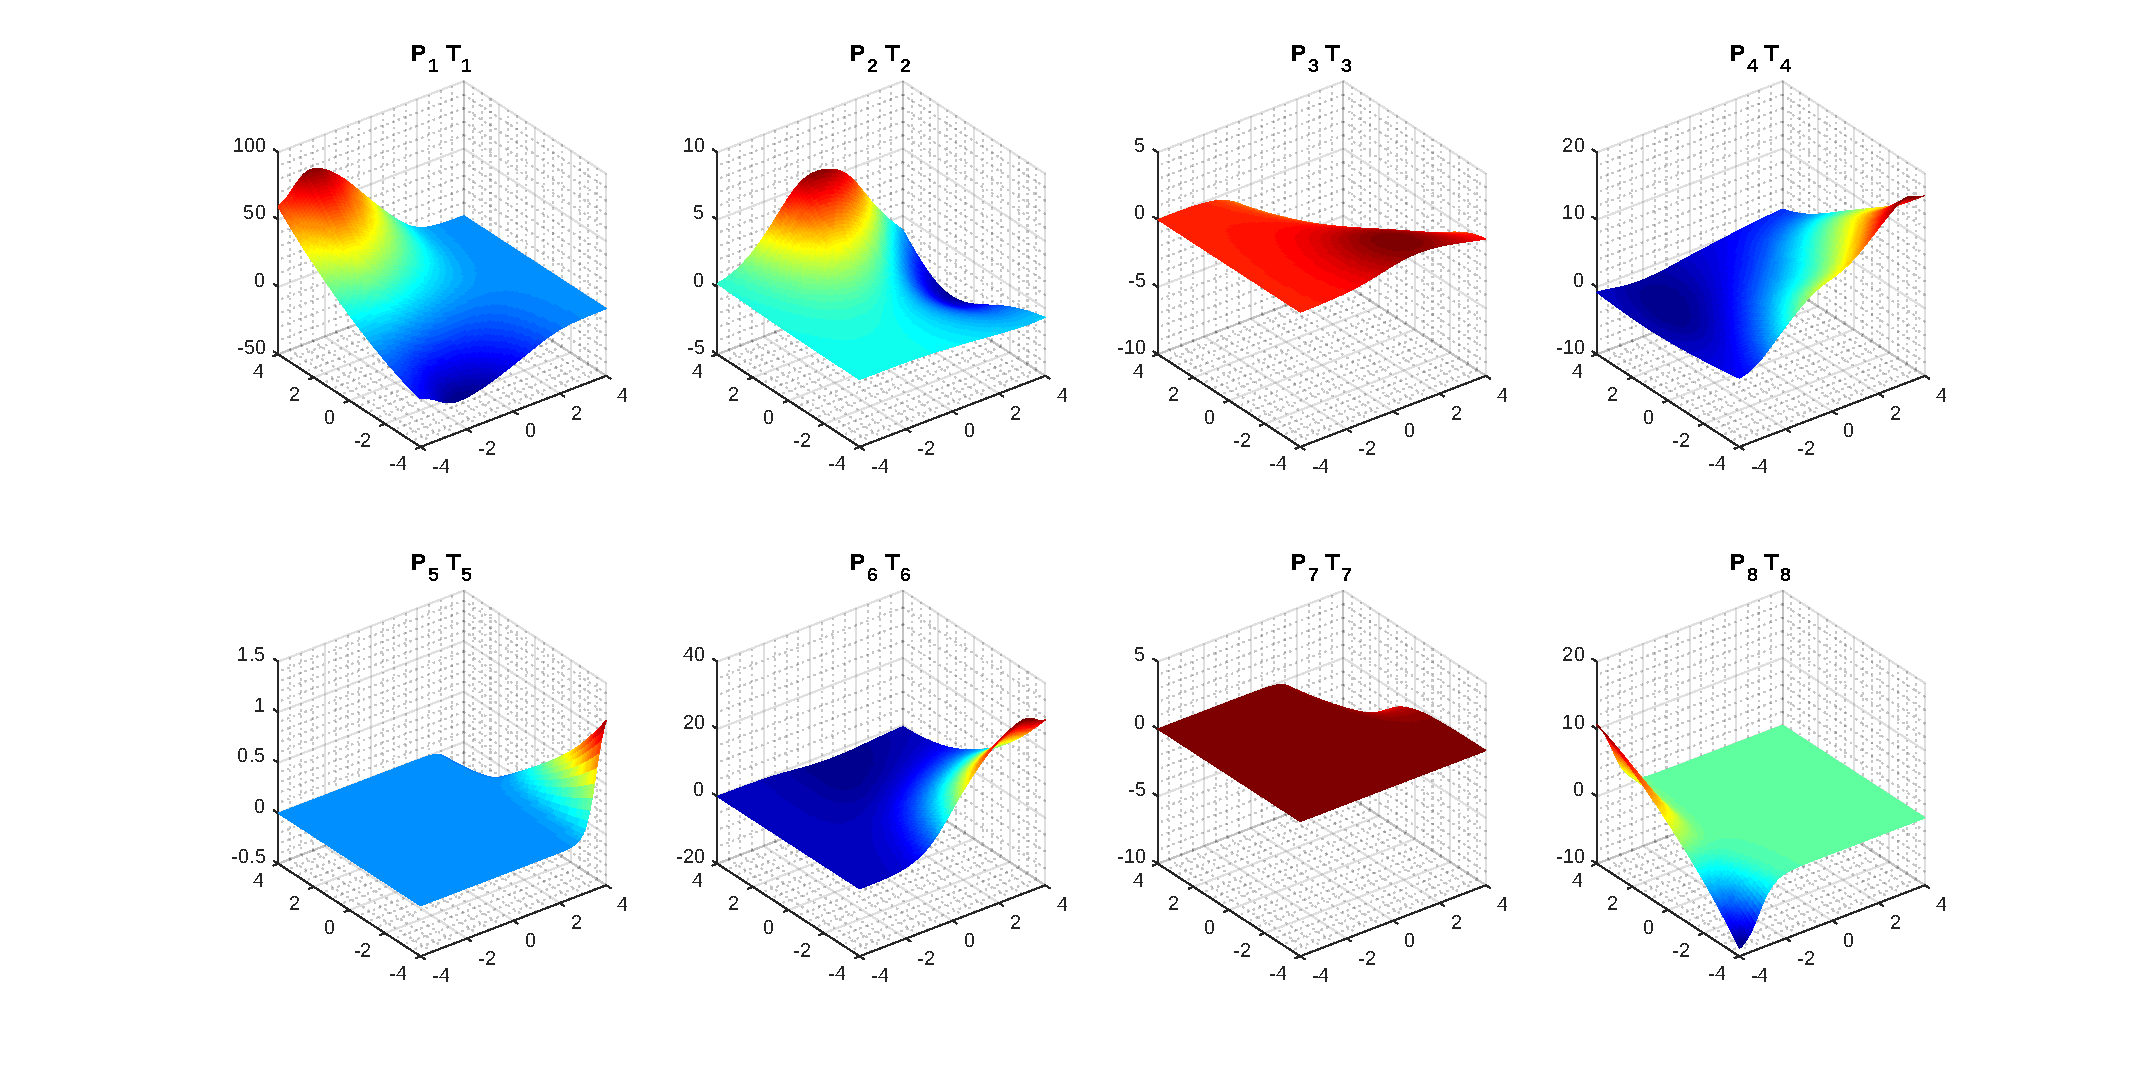
\includegraphics[width=\linewidth]{PT.pdf}
  \caption{Prijenosne funkcije pomnožene pripadnim normiranim težinama.}
\end{figure}

\end{document}
